\documentclass[a4paper,UTF8]{article}
\usepackage{ctex}
\usepackage[margin=1.25in]{geometry}
\usepackage{color}
\usepackage{graphicx}
\usepackage{amssymb}
\usepackage{amsmath}
\usepackage{amsthm}
\usepackage{enumerate}
\usepackage{bm}
\usepackage{hyperref}
\usepackage{epsfig}
\usepackage{color}
\usepackage{mdframed}
\usepackage{lipsum}
\usepackage{mathtools}
\usepackage{algorithm}
\usepackage{algorithmic}
\newmdtheoremenv{thm-box}{myThm}
\newmdtheoremenv{prop-box}{Proposition}
\newmdtheoremenv{def-box}{定义}

\setlength{\evensidemargin}{.25in}
\setlength{\textwidth}{6in}
\setlength{\topmargin}{-0.5in}
\setlength{\topmargin}{-0.5in}
% \setlength{\textheight}{9.5in}
%%%%%%%%%%%%%%%%%%此处用于设置页眉页脚%%%%%%%%%%%%%%%%%%
\usepackage{fancyhdr}                                
\usepackage{lastpage}                                           
\usepackage{layout}                                             
\footskip = 10pt 
\pagestyle{fancy}                    % 设置页眉                 
\lhead{2018年秋季}                    
\chead{高级机器学习}                                                
% \rhead{第\thepage/\pageref{LastPage}页} 
\rhead{作业二}                                                                                               
\cfoot{\thepage}                                                
\renewcommand{\headrulewidth}{1pt}  			%页眉线宽,设为0可以去页眉线
\setlength{\skip\footins}{0.5cm}    			%脚注与正文的距离           
\renewcommand{\footrulewidth}{0pt}  			%页脚线宽,设为0可以去页脚线

\makeatletter 									%设置双线页眉                                        
\def\headrule{{\if@fancyplain\let\headrulewidth\plainheadrulewidth\fi%
\hrule\@height 1.0pt \@width\headwidth\vskip1pt	%上面线为1pt粗  
\hrule\@height 0.5pt\@width\headwidth  			%下面0.5pt粗            
\vskip-2\headrulewidth\vskip-1pt}      			%两条线的距离1pt        
 \vspace{6mm}}     								%双线与下面正文之间的垂直间距              
\makeatother  

%%%%%%%%%%%%%%%%%%%%%%%%%%%%%%%%%%%%%%%%%%%%%%
\numberwithin{equation}{section}
%\usepackage[thmmarks, amsmath, thref]{ntheorem}
\newtheorem{myThm}{myThm}
\newtheorem*{myDef}{Definition}
\newtheorem*{mySol}{Solution}
\newtheorem*{myProof}{Proof}
\newcommand{\indep}{\rotatebox[origin=c]{90}{$\models$}}
\newcommand*\diff{\mathop{}\!\mathrm{d}}

\usepackage{multirow}

%--\right) 

%--
\begin{document}
\title{高级机器学习\\
作业二}
\author{-,-,-}
\maketitle

\section{[30pts] Learning Theory}
\begin{enumerate}[(1)]
	\item \textbf{[10pts] VC维} 

	试讨论最近邻分类器假设空间的VC维大小,并给出证明.
	\item \textbf{[10pts] Rademaher复杂度}
	
	试证明: 常数函数$c$的Rademaher复杂度为$0$.
	\item \textbf{[10pts] PAC} 
	
	$\mathcal{X}=\mathbb{R}^2, \mathcal{Y}= {0,1}.$假设空间$\mathcal{H}$定义如下:$\mathcal{H}=\{h_r:r \in \mathbb{R}_+\}$,其中$h_r (x)=\mathbb{I}(\parallel x \parallel \leq r)$,假定假设空间是可分的,证明$\mathcal{H}$是PAC可学习的,并且样本复杂度为$\frac{log(1/\delta)}{\epsilon}$
	\newline
	(提示:可考虑返回与训练集一致的最小圆的算法)
\end{enumerate}
\begin{myProof}
此处用于写证明(中英文均可)

\begin{enumerate}[(1)]
	\item 记最近邻分类器的假设空间为$\mathcal{H}$,VC维就是该$\mathcal{H}$能打散的数据集的大小。对于最近邻分类器来说,其假设分类是根据距离最近的点的标签进行分类的。所以对任意大的数据集都可以被其假设空间打散,即最近邻分类器的VC维是无限大的。
	\item 假设实值函数空间$\mathcal{F}:\mathcal{Z}\rightarrow\left\{ c \right\}$,令$ \mathrm{Z} =\left\{ \boldsymbol{z}_1, \boldsymbol{z}_2, ..., \boldsymbol{z}_m \right\}$,其中$\boldsymbol{z}_i \in \mathcal{Z}$,则函数空间$\mathcal{F}$关于$\mathrm{Z}$的经验Rademacher复杂度为:
	\[ \hat{R}_Z(\mathcal{F})=\mathbb{E}_{\sigma}\left[ \sup\limits _{f\in\mathcal{F}} \frac{1}{m}\sum_{i=1}^m \sigma_{i}f(\boldsymbol{z}_i) \right] \]
	对于常熟函数$C$有:
	\[ \hat{R}_C(\mathcal{F})=\mathbb{E}_{\sigma}\left[ \frac{1}{m}\sum_{i=1}^m \sigma_{i}C(\boldsymbol{z}_i) \right] \]
	其中$\sigma_i$为随机变量$\sigma$的每一维,以0.5概率取值1,0.5概率取值-1,所以$\mathbb{E}(\sigma_i)=0$,则对应的常数函数$C$的Rademacher复杂度为:
	\[ \begin{aligned}
		\hat{R}_C(\mathcal{F}) &= \mathbb{E}_{\sigma}\left[ \frac{1}{m}\sum_{i=1}^m \sigma_{i}c) \right] \\
		&= c\sum_{i=1}^m \mathbb{E}\left[ \left| \sigma_i \right| \right] \\
		&= 0
	\end{aligned} \]
	\item 假设$\mathcal{X}$里的样本独立同分布于$\mathcal{D}$。假设$h$的泛化误差$E(h)$大于一个非常小的正实数$\epsilon$,则对于分布$\mathcal{D}$上随机采样得到的样例$(x, y)$都有:
	\[ \begin{aligned}
		P(h(x)=y) &= 1 - P(h(x)\neq y) \\
		&= 1 - E(h) \\
		&< 1 - \epsilon
	\end{aligned}\]
	则对于包含$m$个独立样本的训练集$\boldsymbol{D}$来说,假设$h$与其表现一致的概率为:
	\[ \begin{aligned}
		P\Bigl(h(x_1)=y_1)\land\cdots\land h(x_m)=y_m) \Bigr) &= \Bigl(1-P(h(x)\neq y)\Bigr)^m \\
		&= (1 - \epsilon)^m
	\end{aligned} \]
	在保证泛化误差$E(h_r)>\epsilon$且在训练集上的经验误差$\hat{E}(h_r)=0$的假设出现的概率之和不大于$\delta$的情况下有:
	\[ P\Bigl(h\in\mathcal{H}:E(h_r)>\epsilon\land\hat{E}(h_r)=0\Bigr) < \left|\mathcal{H}\right|(1-\epsilon)^m < \left|\mathcal{H}\right|e^{-m\epsilon}\]
	根据题意,$\mathcal{H}=\{h_r:r \in \mathbb{R}_+\}$,其中$h_r (x)=\mathbb{I}(\parallel x \parallel \leq r)$,则输出和训练集一致的最小圆的假设$h_{r**}$即可,其中$r^*$为离原点距离最远的点的距离。那么$\left|\mathcal{H}\right|=1$。则上式可以改写为:
	\[ P\Bigl(h\in\mathcal{H}:E(h_{r^*})>\epsilon\land\hat{E}(h_{r^*})=0\Bigr) < e^{-m\epsilon}\]
	令其不大于$e^{-m\epsilon}\leq\delta$得$m\ge\frac{\ln(1/\delta)}{\epsilon}$。

	综上,$\mathcal{H}$是PAC可学习的,并且样本复杂度为$\frac{log(1/\delta)}{\epsilon}$
\end{enumerate}

\end{myProof}
\newpage

\section{[30pts] 文档主题模型}
在一个新闻数据集上实现文档主题模型(Latent Dirichlet Allocation~(LDA))~\cite{DBLP:journals/jmlr/BleiNJ03}.

我们提供了一个包含8,888条新闻的数据集,请在该数据集上完成LDA算法的使用及实现。

\begin{itemize}
	\item 数据集下载:\href{http://lamda.nju.edu.cn/ml2018grad/dataset/news.txt.zip}{新闻数据集.}
	\item 格式:每行是一条新闻.
\end{itemize}

数据预处理提示:你可能需要完成分词及去掉一些停用词等预处理工作.

\begin{enumerate}[(1)]
	\item \textbf{[10pts] 任务\#1:使用LDA模型} 
	\subitem A. 选择开源的LDA库(例如:\href{https://scikit-learn.org/stable/modules/generated/sklearn.decomposition.LatentDirichletAllocation.html}{scikit-learn}),并在提供的数据集上学习使用.
	\subitem B. 给出$K=\{5,10,20\}$个主题时,每个主题下概率最大的$M=10$个词及其概率.
	\item \textbf{[20pts] 任务\#2:实现LDA模型} 
	\subitem A. 不借助开源库,自己完成LDA算法.
	\subitem B. 给出$K=\{5,10,20\}$个主题时,每个主题下概率最大的$M=10$个词及其概率.
\end{enumerate}
\begin{mySol} 
	
	无论是调库还是调库,首先都要对数据进行预处理。我的预处理规则如算法1:需要说明的是停用词是在网上找的常见,结合nltk库自带的,两者加起来共900多个。nltk本身只有100多个停用词。
	
	在和其他同学交流的时候发现数据处理部分不同的人有不同的理解,主要有:
	\begin{itemize}
		\item[1)] 某些词是否算停用词,例如我认为dr(Dr), ms(Miss.), mr(Mr), mrs(Mrs)等都算停用词,但有些同学认为不是。
		\item[2)] 数字问题,我认为只要带有数字的词都应该去掉,例如年份,次数(如1st),有些同学认为这些数字词本身也应该作为分类的依据之一。
	\end{itemize}

	\begin{algorithm}[htb]
		\caption{ 数据预处理规则 }
		\label{alg1}
		\hspace*{0.02in}{\textbf{Input:}} \\
		原始文档$news.txt$ \\
		停用词$stop\_words.txt$ \\
		\hspace*{0.02in}{\textbf{Output:}} \\
		处理后的文档$pre\_news.txt$ \\
		词-id映射$wordmapid$
		\begin{algorithmic}[1]
			\STATE { 读取停用词表$stop\_words.txt$ $\to$ stopword }
			\STATE { 读取原始文档$news.txt$ }
			\FOR{ 文件里的每一行,即每一条新闻 }
				\FOR{ 一行新闻里的每个词 }
					\STATE { 全部转换成小写字母 }
					\STATE { 去掉标点符号,即将标点符号替换成空字符 }
					\STATE { 去掉带有数字的词 }
					\STATE { 去掉停用词 }
					\STATE { 为每个词创建一个id,根据他们出现的次序递增}
				\ENDFOR
				\STATE { 组成新句子并写入文件$pre\_news.txt$(追加) }
			\ENDFOR
			\STATE {将全部词-id映射写入文件wordmapid}
		\end{algorithmic}
	\end{algorithm}

	调库使用sklearn库,参考了两个博客链接:
	\begin{itemize}
		\item[1)] \href{https://blog.csdn.net/TiffanyRabbit/article/details/76445909}{【sklearn】利用sklearn训练LDA主题模型及调参详解}
		\item[2)] \href{https://www.cnblogs.com/pinard/p/6908150.html}{用scikit-learn学习LDA主题模型}
	\end{itemize}
	
	实现LDA模型(非调库)的代码参考了一个技术博客和一些理论讲解博客,在此只列出参考的技术博客:
	\begin{itemize}
		\item[1)] \href{https://www.cnblogs.com/wang2825/articles/8687889.html}{LDA之主题模型原理解析与python实现}
	\end{itemize}

	实现LDA模型主要涉及两个算法,算法2: LDA模型变量的初始化 以及 算法3: sampling抽样:

	\newpage
	\begin{algorithm}[!htb]
		\caption{ LDA模型变量的初始化 }
		\label{alg2}
		\hspace*{0.02in}{\textbf{Input:}} \\
			处理后的文档$pre\_news.txt$, 词-id映射规则$wordmapid$ \\
			分类个数$K$ \\
		\hspace*{0.02in}{\textbf{Output:}}
			随机分派了一次的LDA模型
		\begin{algorithmic}[1]
			\STATE { init $p$: $size=(K,)$ }
			\STATE { init $nw$: $size=(M, K)$, 表示词在类上的分布,其中M为词的总数 }
			\STATE { init $nwsum$: $size=(K,)$, 表示每个类上词的总数 }
			\STATE { init $nd$: $size=(N, K)$, 表示每个类中词的分布,其中N为文章数量 }
			\STATE { init $ndsum$: $size=(N,)$, 表示每篇文章中词的个数 }
			\STATE { init $Z$: $size=(N, W)$, 表示每个词分派的一个类,其中W为每篇文章中词的个数 }
			\STATE { init $topK$: $size=(N, K)$, 最终计算的文章-类的概率分布 }
			\STATE { init $topW$: $size=(K, M)$, 最终计算的类-词的概率分布 }
			\STATE { 随机初始化分派类 }
			\FOR{ 1,2,$\cdots$,V }
				\STATE { 统计$ndsum$[文章id][词的个数] }
				\FOR{ 1,2,$\cdots$,W }
					\STATE { 为每个词随机分派一个类 }
					\STATE { 词在此主题上的分布数目+1 }
					\STATE { 此文章中此主题上的词的个数+1 }
					\STATE { 此主题的总词数+1 }
				\ENDFOR
			\ENDFOR
		\end{algorithmic}
	\end{algorithm}

	\newpage
	\begin{algorithm}[!htb]
		\caption{ sampling抽样 }
		\label{alg3}
		\hspace*{0.02in}{\textbf{Input:}}
			初始化后的LDA模型 \\
		  	迭代次数iter-times \\
		  	超参数$\alpha$, $\beta$ \\
			分类个数$K$ \\ 
		\hspace*{0.02in}{\textbf{Output:}}
			LDA模型,大体有以下三项:\\
			topK, 文档-主题概率分布 \\
			topW, 主题-词概率分布 \\
			topM, 每个类中topM个词
		\begin{algorithmic}[1]
			\STATE { init $p$: $size=(K,)$ }
			\STATE { init $nw$: $size=(M, K)$, 表示词在类上的分布,其中M为词的总数 }
			\STATE { init $nwsum$: $size=(K,)$, 表示每个类上词的总数 }
			\STATE { init $nd$: $size=(N, K)$, 表示每个类中词的分布,其中N为文章数量 }
			\STATE { init $ndsum$: $size=(N,)$, 表示每篇文章中词的个数 }
			\STATE { init $Z$: $size=(N, W)$, 表示每个词分派的一个类,其中W为每篇文章中词的个数 }
			\STATE { init $topK$: $size=(N, K)$, 最终计算的文章-类的概率分布 }
			\STATE { init $topW$: $size=(K, M)$, 最终计算的类-词的概率分布 }
			\STATE { 随机初始化分派类 }
			\FOR{ i in 1,2,$\cdots$,iter-times(迭代次数) }
				\FOR{ m in 1,2,$\cdots$,N(文章数) }
					\FOR{ n in 1,2,$\cdots$,W(每篇文章中词的个数) }
						\STATE { topic = Z[m][v] }
						\STATE { nw[v][topic]++、nwsum[topic]++、nd[m][topic]++  }
						\STATE { 计算此词属于每个topic的概率p; }
						\FOR{ k in 1,2,$\cdots$,K-1(类的个数) }
							\STATE { p[k] += p[k-1] }
							\STATE { 再随机分派一次,记录被分派的新的topic }
							\STATE { nw[v][new-topic]++、nwsum[new-topic]++、nd[m][new-topic]++	}
						\ENDFOR
					\ENDFOR
				\ENDFOR
			\ENDFOR
		\end{algorithmic}
	\end{algorithm}

	关于代码文件的说明,详细看README.md文档。实验结果文件,命名方式为 \\
		``self/sklearn\_lda\_K\%dM\%d\_iter\%d" \% (K, M, iter\_times),其中:

	self表示非调库实现的LDA,sklearn表示使用sklearn的LDA;

	$K$是主题数,取值有$K=[5, 10, 20]$;

	$M$是每个主题下概率最大的$M$个词,题目要求$M=10$,也可以在程序中改成其他值;
	
	$iter\_time$表示迭代次数,代码中默认设置为$iter\_times=100$,通过理论以及经过实验可以知道,迭代次数不宜太小,否则分类结果很差,例如在验证程序是否有误的时候我曾试过将该值设为1,那么分类出来的结果,每类下的topM个词都差不多是同样的词。 \\
	
	和几个同学对比了一下,虽然每个分类的词不一样,即使词一样,概率也不一样,但是还是能分辨出两份结果分的类是一致的。例如k=5的时候明显有一类是和美国总统有关的(我猜应该是选举),government、president等的词可以分辨出,这些词倒是都会出现,只是概率不同而已。有些同学的结果出现obama,有些出现trump,通过这些能大胆推测是同一类的。\\

\end{mySol}

\newpage
\ \\
\newpage

\section{[40pts] 强化学习实验}
用DQN (deep Q Networks) 训练Flappy Bird. 请各位同学根据DQN算法流程,补全提供的代码包中\text{deep\_q\_networkd.py}文件中“\# TODO”部分代码 (补全 epsilon-greedy action selection以及Q learning updating),了解DQN算法,并进行训练,本实验时间相对较久.

本次实验所需要的依赖如下:
\begin{itemize}
	\item python2.7 or python3;
	\item pygame;
	\item OpenCV-python;
	\item TensorFlow (建议使用1.1-1.6).
\end{itemize}

强化学习中经典的off-policy算法Q-Learning的原始版本采用表格形式来记录$Q$函数,显然只能应用于有限离散状态、有限离散动作且状态、动作数量较少的情况下,即有维度灾难问题 (表格大小正比于 $|S|*|A|$). 采用函数近似法,假定$Q$函数可由状态特征经过某个函数的映射到对应动作的评价值上,可扩大Q-Learning使用范围. 近年来,DeepMind结合深度模型强大的表达能力,用深度神经网络作为近似函数来表达强化学习中的 $Q$ 函数,进一步扩大了Q-Learning可用范围. DQN中采用experience replay和target network两种技术,使DQN的训练更加高效且鲁棒,并在atari的部分游戏上取得了人类水平的表现.

DQN的流程大致如下~\ref{alg:DQN}:
\begin{algorithm}
	\caption{DQN with experience replay}
	\label{alg:DQN}
	\begin{algorithmic}
		\STATE {Initialize replay memory $D$ to capacity $N$} 
		\STATE {Initialize action-value function $Q$ with random weights $\theta$}
		\STATE {Initialize target action-value function $\hat{Q}$ with weights $\theta^- =\theta$}
		\FOR{$episode=1,M$}
		\STATE {Initialize sequence $s_1={x_1}$ and preprocessed sequence $\phi_1=\phi(s_1)$}
		\FOR{$t=1,T$}
		\STATE {With probability $\epsilon$ select a random action $a_t$}
		\STATE {otherwise select $a_t=\arg\max_a Q(\phi(s_t),a;\theta)$}
		\STATE {Execute action $a_t$ in emulator and observe reward $r_t$ and image $x_{t+1}$}
		\STATE {Set $s_{t+1}=s_t,a_t,x_{t+1}$ and preprocess $\phi_{t+1}=\phi(s_{t+1})$}
		\STATE {Store transition $(\phi_t,a_t,r_t,\phi_t)$ in $D$}
		\STATE {Sample random minibatch of transitions $(\phi_j,a_j,r_j,\phi_{j+1})$ from $D$}
		\STATE {Set 
			\begin{equation}
			f(x)=
			\begin{cases}
			r_j& \text{if episode terminates at step $j+1$}\\
			r_j+\gamma\max_{a'}\hat{Q}(\phi_{j=1},a';\theta^-)& \text{otherwise}
			\end{cases}
			\end{equation}}
		\STATE {Perform a gradient descent step on $(y_j-Q(\phi_j,a_j;\theta))^2$ with respect to the network parameters $\theta$}
		\STATE {Every $C$ steps reset $\hat{Q}=Q$}
		\ENDFOR
		\ENDFOR
	\end{algorithmic}
\end{algorithm}

上图是15年DeepMind发表在Nature上文章中所采用的算法流程,包含了 experience replay和target network技术,本次实验不要实现target network ,仅需要实现experience replay即可 (实现target network可额外获得$5$pts bonus). 感兴趣的同学可参阅DQN相关教程或文章,进一步了解两种技术. 

本次实验中状态太输入为raw pixel,转为$80*80$的灰度图 (采用openCV转换),并将历史最近$3$个frame叠加到当前frame中作为状态输入,即每一步输入状态为$4*80*80$,动作为$2$维离散动作 (上、下,action为$2$维one-hot编码). 网络模型已经搭建好 (采用TensorFlow 搭建),输入为$4*80*80$,输出为$2$,对应每个动作对应的 $Q$ 值。如下图所示~\ref{fig:rl_1}.
\begin{figure}[!htb]
	\centering
	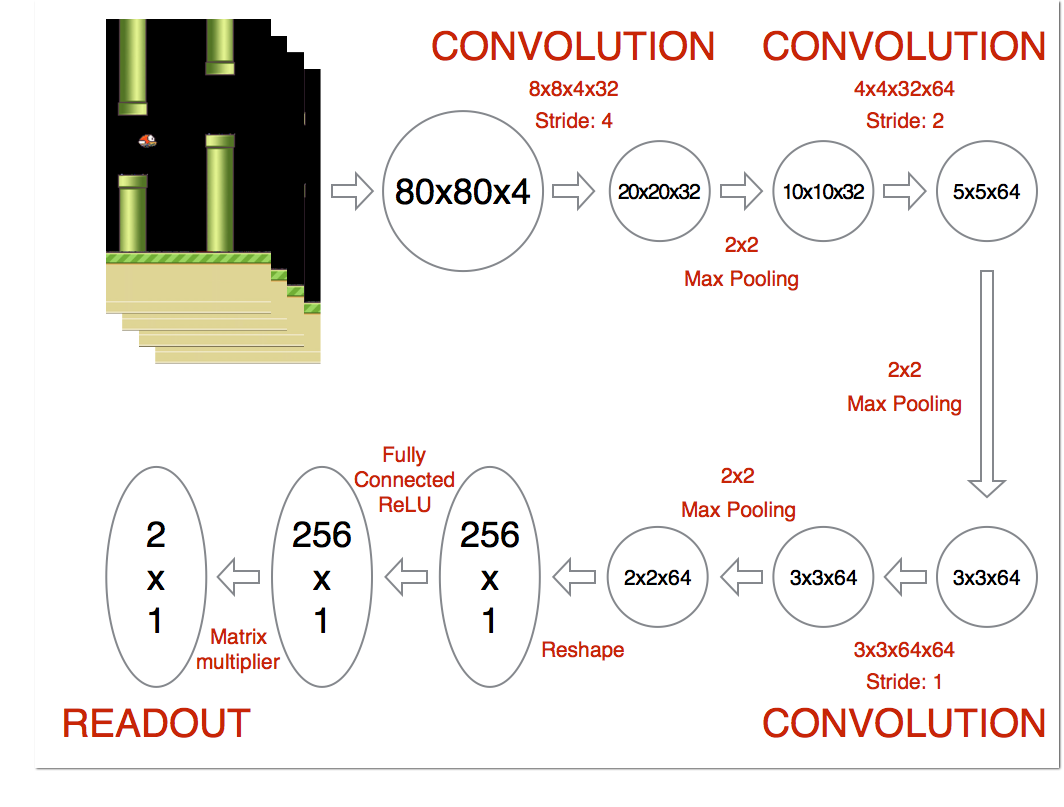
\includegraphics[scale=0.4]{rl_1.png}
	\caption{网络模型.}
	\label{fig:rl_1}
\end{figure}

游戏环境中,单步奖励为$0.1$,越过一个管道$+1$,死亡得到$-1$的惩罚. 可采用其他深度学习框架,如 pytorch、keras 等搭建模型并完成训练代码. DQN算法设置可采用如下配置:
\begin{itemize}
	\item GAMMA = 0.99 \# decay rate of past observations;
	\item OBSERVE = 10000. \# timesteps to observe before training;
	\item EXPLORE = 2000000. \# frames over which to anneal epsilon;
	\item FINAL\_EPSILON = 0.0001 \# final value of epsilon;
	\item INITIAL\_EPSILON = 0.1~0.2 \# starting value of epsilon;
	\item REPLAY\_MEMORY = 50000 \# number of previous transitions to remember;
	\item BATCH = 32 \# size of minibatch;
	\item FRAME\_PER\_ACTION = 1.
\end{itemize}

默认一直训练不会终止,每$10,000$ frames保存一个模型,默认最大保存$5$个,保存的模型可恢复用来测试,默认保存在save\_model 目录下. 采用GPU可加速训练,仅使用双核CPU训练时,采用如上配置,总样本量到$1$M ($1,000,000$个state) 需要时间为$20$~$24$h,大概$3$M可训练出相当不错的策略,考虑到计算咨询和时间,可自行选择训练量.

采用其他深度学习框架时,只需要保持从环境中获得返回的状态、奖励信息,以及是否终止,并可在环境中执行action (再次注意,action为$2$维one-hot编码). Agent与环境交互过程如下所示:
\begin{itemize}
	\item sys.path.append("game/");
	\item import wrapped\_flappy\_bird as game \# import game environment;
	\item game\_state = game.GameState() \# initialize;
	\item \# execute an action and get info from the environment;
	\item $x_t, r_0$, terminal = game\_state.frame\_step(action).
\end{itemize}

本实验提交要求:

仅需提供补全后deep\_q\_network.py文件,以及训练后的短视频 (连续飞行$5-10$s 即可) 或图片或gif动图等辅助证明材料,并说明训练使用样本量. 如果有任何修改或补充说明,请一并说明. (建议写Readme文件或报告)



\begin{mySol}
此处用于写解答(中英文均可)

实验每10000次存储一个模型文件,并且只保留最新的5个(即最近50000次),实验在windows下运行,至少跑了2840000次。录制了51秒的视频,文件名为$Flappy Bird 2018\_12\_20 10\_18\_26.mp4$。代码参考了\url{https://github.com/yenchenlin/DeepLearningFlappyBird}

\end{mySol}
\newpage


\bibliographystyle{plain}
\bibliography{ref}
\end{document}